\documentclass[a4paper,11pt]{article}
\usepackage[utf8]{inputenc}
\usepackage[OT1]{fontenc}
\usepackage[english]{babel}
\usepackage[margin=1.2in]{geometry}
\usepackage{graphicx}
\usepackage{amsmath}
\usepackage{cite}

\usepackage{pslatex}

%\usepackage{fancyvrb}

\author{Simon Mitternacht}
\date{\today}
\title{Sasalib Manual}

\begin{document}
\maketitle
\noindent
The program/library Sasalib, including this manual, is licensed under
GPLv3, and can be downloaded from the github at: 
\begin{center}
\texttt{https://github.com/mittinatten/sasalib/}
\end{center}

This document is still a draft and not complete in any way.

\newpage
\section{Introduction}

Sasalib is a program for calculating solvent accessible surface areas
(SASA) for proteins. It can both be used as a standalone command line
program or as a C library. The library interface allows the user to
set most parameters of the calculation, and returns the SASA of the
individual atoms, allowing summation of SASA over user-defined
atom-classes. The library provides both the Lee \& Richards
\cite{LnR} and Shrake \& Rupley \cite{SnR} algorithms.

To the author's knowledge there aren't any fully open source programs for
calculating solvent accessible surface areas (SASA) of
proteins. Neither are there any packages designed to be easily
integrated as a library in other programs. 

The SASA is defined as the surface area of a protein accessible to a
spherical probe rolling over the protein, including internal
cavities. The probe represents a solvent molecule (i.e. water), and
therefore cavities that are too small for the solvent to enter are not
counted at all. The position of the center of the probe sphere is used
to define the surface area, not the point of contact.

\section{Getting started}

The following shows a minimal program that performs a SASA-calculation
using a PDB-file as input. No error checking is done, the example
simply illustrates the most basic functionality of the library.
\begin{verbatim}
#include <stdlib.h>
#include <sasalib.h> // if in include-path

int main(int argc, char **argv) { 
    //initialize sasalib-object with default parameters
    sasalib_t *s = sasalib_init();

    //do the calculation using default parameters with protein
    //structure from STDIN
    sasalib_calc_pdb(s,stdin);

    sasalib_print(stdout,s);     //print results to STDOUT

    //clean up
    sasalib_free(s);

    return EXIT_SUCCESS;
}
\end{verbatim}
The output of the program is (using the structure with PDB code 1UBQ):
\begin{verbatim}
name: undef
algorithm: Shrake & Rupley
N_testpoint: 100
time_elapsed: 0.018549 s
n_atoms: 602

> polar_apolar
apolar   2788.07
polar   1968.06

> all
total   4756.12
\end{verbatim}
The first 3 lines show the name of the protein, the algorithm and the
parameters of the algorithm (the ones shown here are default
values). Then comes data over calculation time and the size of the
protein. Each result begins with \texttt{>} followed by the grouping
of atoms used. The label \texttt{polar\_apolar} means that the atoms
have been divided into polar and apolar atoms (based on Ooi et
al. \cite{OONS}). The SASA values are given in Å$^2$.

\section{Algorithms}

There are two classical approximate algorithms that can be used to
calculate SASA, by Lee \& Richards \cite{LnR} and Shrake \& Rupley
respectively \cite{SnR}. Both can be calculated to arbitrary precision
by refining the resolution.

We will use the following notation: An atom $i$ has a van der Waals
radius $r_i$, the surface probe has radius $r_\text{P}$ and when these
are added we get $R_i = r_i + r_\text{P}$. The SASA is calculated by
adding up the surface patches of the spheres of radius $R_i$ that are
not overlapping with any other sphere.

\subsection{Lee \& Richards} \label{sec:alg_LnR}

Lee \& Richards' algorithm calculates the surface area by slicing the
protein, calculating the length of the solvent exposed contours in
each slice and then adding up the length multiplied by the slice
thickness. Precision is increased by making the slices thinner and the
calculation time scales as the number of slices.

Divide the protein into slices of thickness $\delta$ along an
arbitrary axis. The position of the slice along that axis is denoted
$z$. The position of the center of atom $i$ along the same axis is
$z_i$. In the slice, each atom is thus a circle of radius $$R_i^\prime
= \sqrt{R_i^2-(z-z_i)^2}\,.$$ These circles are either completely buried,
completely exposed, or partially exposed.

The exposed arc lengths for each atom can be calculated exactly. For
each pair of atoms $i,j$, the distance between their centers is
$d_{ij}$. If $d_{ij} > R_i^\prime + R_j^\prime$, there is no
overlap. If $d_{ij} < R_j^\prime - R_i^\prime$ circle $i$ is
completely inside $j$, and the other way around. If $d_{ij}$ lies
between these two cases the angle of circle $i$ that is buried due to
circle $j$ is $$\alpha = 2\arccos \bigl[({R_i^\prime}^2 + d_{ij}^2 -
  {R_{j}^\prime}^2)/(2R_i^\prime d_{ij})\bigr].$$ The middle point of
the arc on the circle is at an angle $\beta$ in circle $i$, and thus the
arc spans the interval $[\beta-\alpha/2,\beta+\alpha/2]$. By adding up
these arcs and taking into account any overlap between them we get
the total buried angle $\gamma_i$ of circle $i$. The exposed arc length in
this slice is thus $L_i = R_i^\prime(2\pi-\gamma_i)$.

The contribution to the SASA from each slice is $$ S_\delta =
\sum_{i \in \text{slice}}L_i\Delta_i $$ where
$$
  \Delta_i = \frac{R_i}{R_i^\prime} \biggl[\frac{\delta}{2} 
    + \min\biggl(\frac{\delta}{2},R_i -
    \lvert z - z_i \rvert\biggr)\biggr]. 
$$ 
Finally, the total SASA is obtained by adding up the contribution from
all the slices, either for the whole protein, or atom by atom.

\subsection{Shrake \& Rupley}

For each atom $i$, use a set of test points evenly distributed
(approximately) over the sphere of radius $R_i$, and count how many of
the test points are not inside any of the other extended spheres of
radius $R_j$. The number of exposed testpoints divided by the total
number of test points gives the exposed solid angle of that atom. The
precision of the algorithm is increased by increasing the number of
test points, and calculation time scales linearly with the number of
test points.

The test points used in Sasalib were generated by placing a set of
equal point charges on the surface of a sphere and minimizing the Coulomb
potential (using simulated annealing).

\subsection{Comparison of the two}

\subsubsection{Dataset}

For evaluating and comparing the two algorithms a list of proteins was
downloaded from the PISCES server (on Aug 12, 2013). The proteins have
less than 20\,\% sequence identity, and the structures a resolution of
1.6~Å or less and R-factors less than 0.25. The list specifies which
chain to use in a specific PDB-file. For the calculations here, whole
PDB-files are used, giving a larger variation in protein size, which
is useful for our purposes. The 2117 chains in the list gave a set of
2056 protein structures used for all calculations below.

\subsubsection{Speed}

In the limit of low precision the calculation time will be limited by
the time it takes to find which atoms are neighbours, which scales as
the square of the number of atoms. This calculation can be linearized,
but with a relatively large constant, making it worthwhile only for
large proteins. (Do more tests here?)

In the limit of high precision the calculation time of both algorithms
will instead scale as the number of atoms: If the number of
test-points is large in S\&R, most of the time will be spent
calculating the overlap, instead of which atoms are in contact. If
there are many slices in L\&R, the calculation time will be
proportional to the number of slices, and the time of each
slice linear in the number of atoms in the slice. 

The point where the calculation time crosses over from linear to
quadratic in the number of atoms thus depends on the precision as
figure~\ref{fig:time} shows. The same figure also shows that there is
more variation in time needed for S\&R than for L\&R, which is
probably because the S\&R is more sensitive to the density of the
protein than the L\&R. L\&R is mainly limited by the number of slices
and the number of atoms in the slice, with a smaller cost of actually
analyzing the overlap between atoms in each slice, wheras the
calculation in S\&R is completely dominated by the number of overlaps
that are calculated. The fact that the effect is largest for the case
with the most test points supports this interpretation.

\begin{figure}
  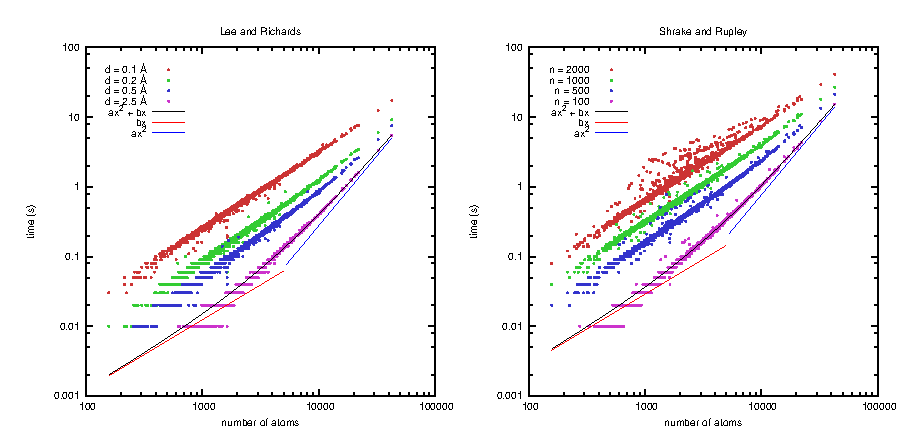
\includegraphics{../analysis/plots/time}
  \caption{Calculation time as function of number of atoms for
    different levels of precision. In both cases the cross-over from
    linear to quadratic scaling as function of protein size is only
    clearly visible for the lowest precision used. The discretization
    is because time was measured with a precision of 1
    ms.\label{fig:time}}
\end{figure}

\subsubsection{Accuracy as function of speed}\label{sec:accuracy}

To measure accuracy of the two algorithms a reference SASA value,
$S_\text{ref}$ was calculated using L\&R with slice thickness
0.001~Å. The error of a given SASA-value, $S$ is then $\delta = \lvert
S - S_\text{ref} \rvert / N$, where $N$ is the number of atoms in the
protein. Figure~\ref{fig:precision} shows the results of these
calculations for the 2056 proteins described above. In accordance with
figure~\ref{fig:time} S\&R gives a more varied behavior than L\&R,
i.e. a broader distribution of values. It is clear from this picture
that S\&R is on average an order of magnitude more accurate than L\&R
given the same computational effort -- in the present implementation.

\begin{figure}
  \begin{center}
  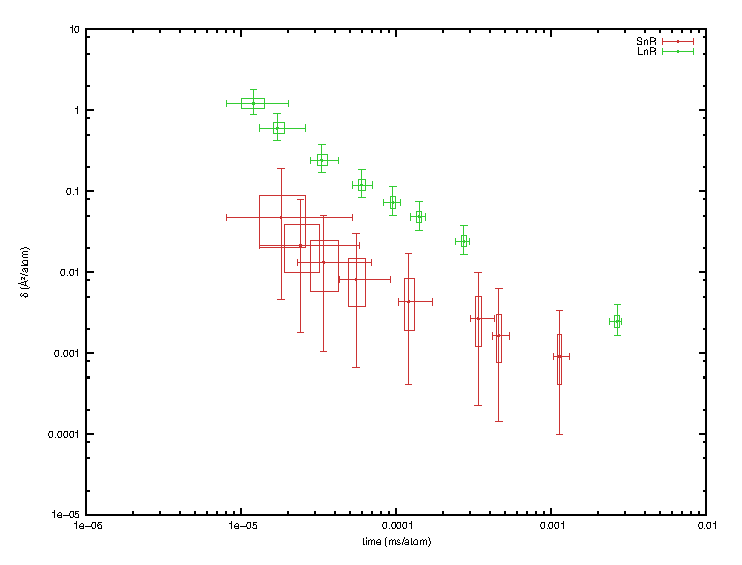
\includegraphics{../analysis/plots/precision}
  \caption{The error $\delta$ in calculated SASA vs calculation time
    $t$ for the two algorithms. For the different S\&R calculations
    20, 50, 100, 200, 500, 1000, 2000 and 5000 test points were
    used. For L\&R slice thicknesses 0.01, 0.1, 0.2, 0.3, 0.5, 1.0,
    2.5 and 5.0 Å. The borders of the boxes indicate the quartiles of
    the distribution of $t$ and $\delta$ (i.e. 50~\% of the data are
    within the box), and the error bars 5th and 95th percentiles.
    \label{fig:precision}}
  \end{center}
\end{figure}


\section{Implementation}

This section describes the implementation of the algorithms in general
terms. For the library and command-line interfaces see section
\ref{sec:using}. In both cases the implementations are rather
straightforward keeping the implementation rather simple and
transparent.

\subsection{Lee \& Richards}

The L\&R-calculation needs to know which atoms make contacts for each
slice. Therefore the calculation begins by constructing adjacency
lists for the protein. An contact matrix was used in early versions of
the library, but the $O(N^2)$ memory requirements were prohibitive for
large proteins. For each slice the adjacency lists are condensed to
separate lists only containing the atoms in that particular
slice. Each pair of adjacent atoms is then checked for adjacency in
the particular slice and the overlapping arcs are calculated as
described in section \ref{sec:alg_LnR}. When all buried arcs are
counted for a given atom they are reduced to non-overlapping intervals
recursively. In most cases this is done in one step, sometimes in two
or three. The arc-lengths are then summed up for all atoms in the
slice to calculate the total contribution to the area as described in
\ref{sec:alg_LnR}.

As described in section \ref{sec:accuracy}, this algorithm is
significantly slower than S\&R, but this is inherent to the algorithm
[references??]. Profiling runs give no hints at obvious
improvements. The calculations can however be trivially parallelized
by calculating each slice in a separate thread, similar improvements
can be achieved by treating atoms separately in S\&R.

\subsection{Shrake \& Rupley}



\section{Using Sasalib} \label{sec:using}

\subsection{Installing}

The repository can be cloned from the github either using git directly
with the command
\begin{verbatim}
    $ git clone https://github.com/mittinatten/sasalib.git
\end{verbatim}
or by downloading the zipped archive from
\begin{verbatim}
    https://github.com/mittinatten/sasalib/archive/master.zip
\end{verbatim}
Since Sasalib only depends on regular C and GNU libraries most users
will be able to compile it by simply typing \texttt{make}\footnote{Has
  been tested on Linux and Mac OS X machines.}. If any other compiler
than the Gnu C Compiler is preferred the makefile will need to be
changed accordingly.

\subsection{Stand-alone program}

Compilation creates the binary \texttt{calc\_sasa}, which can be used
to calculate the SASA of a PDB-file. The simplest program call, with
default parameters would be
\begin{verbatim}
    $ calc_sasa PDB-file
\end{verbatim}
Or, from STDIN:
\begin{verbatim} 
    $ calc_sasa < PDB-file    
\end{verbatim}
STDIN is only read if no file is specified.

Other options for running are displayed with the flag
\texttt{-h}. These options allow the user to specify which algorithm
to use, and parameters for the algorithm. By default the Shrake \&
Rupley algorithm is used, with 100 test points. This option gives a
fast calculation, for high precision the number of test points should
be increased. The following uses Lee \& Richards with slice width 0.1 Å
for two PDB-files.
\begin{verbatim}
    $ calc_sasa -L -d 0.1 1abc.pdb 2abc.pdb
\end{verbatim}

\subsection{Library interface}

Sasalib provides functions for doing the following steps in a SASA
calculation:
\begin{enumerate}
  \item Initialize protein.
  \item Calculate atomic radii.
  \item Calculate SASA.
  \item Output results grouping atoms/residues in different ways.
\end{enumerate}
The third step is the core functionality of the library and can be
used separately if users wish to handle the other steps
themselves. Below follows a brief description for the functionality
provided for each of the four steps, but first a sample program
showing a complete workflow.

\subsubsection{Sample program}
The following lines read a PDB-structure from a file, calculates
SASA using Lee \& Richards' algorithm and outputs the values for the
polar and apolar atoms respectively.
\begin{verbatim}
#include <stdio.h>
#include <stdlib.h>
#include "protein.h"
#include "sasa.h"

int main(int argc, char **argv) {
    // initialization from STDIN
    protein *p = protein_init_from_pdb(stdin);

    // allocate memory
    double *sasa = (double*) malloc(sizeof(double)*protein_n(p));
    double *r = (double*) malloc(sizeof(double)*protein_n(p));

    // calculate atomic radii
    protein_r_def(p,r);
    
    // SASA calculation using Lee & Richards with 
    // slices of width 0.25 Å
    sasa_lee_richards(sasa,protein_xyz(p),r,protein_n(p),0.25);

    // Output SASA for polar/apolar atoms
    sasa_per_atomclass(stdout,oons_classes(),p,sasa);
   
    // free memory
    protein_free(p);
    free(sasa);
    free(r);

    return 0;
}
\end{verbatim}

\subsubsection{Initiate a protein}

A protein is represented by the struct \texttt{protein}, which is
declared in the header \texttt{protein.h}. A proteins can be
initialized either by reading a PDB-file or by adding atoms manually
one-by-one.

The following function initializes a protein from a PDB-file
\begin{verbatim}
    protein* protein_init_from_pdb(FILE*); 
\end{verbatim}
The pointer is freed using
\begin{verbatim}
    void protein_free(protein*);
\end{verbatim}
An empty protein struct is allocated with 
\begin{verbatim}
    protein* protein_init();
\end{verbatim}
which can then be used to add atoms one by one
\begin{verbatim}
    void protein_add_atom(protein *p, 
                          const char* atom_name,
                          const char* residue_name, 
                          const char* residue_number,
                          char chain_label,
                          double x, double y, double z);

\end{verbatim}
for example like this
\begin{verbatim}
    protein *p = protein_init();
    protein_add_atom(p, " CA ", "GLY", "   1", "A",
                     x, y, z);
\end{verbatim}
Here the labels for the atom are as they would be in a PDB file,
including whitespace. The atom name is a 4-character string, like the
second argument above, the residue name a 3-character string, like the
third argument, the residue number has 4 characters, and the chain
label 1. The last three arguments are the coordinates of the atom. The
reason residue numbers are not represented as integers here, is that
in some PDB files have number sequences such as 1A, 1B, 1C, 1D, 2, 3,
4, \ldots.

The rationale for directly using the strings found in PDB files is
twofold. (i) Most programs that handle proteins will have routines for
generating PDB-files and it should thus be fairly straightforward to
integrate this library into such a program. (ii) Non-standard atoms
can be added with the labels they have in the input, making
sub-sequent analysis more straightforward. This means that no analysis
is performed of the atom types, to check for consistency, etc. The
atom types are only used later for assigning radii to the atoms,
something that can also be done manually.

\subsubsection{Assign atomic radii}
Give each atom a radius. Sasalib can calculate atomic radii according
to Ooi et al (OONS-radii) for the 20 canonical amino acid types. The
user can also specify the radius for each individual atom. The two
methods can be combined if a protein has a few non-standard atoms.

Functions for OONS-classification are found in \texttt{oons.h}. There
are two versions
\begin{verbatim}
    double oons_radius_pdbline(const char *pdb_line);
    double oons_radius(const char *res_name,
                       const char *atom_name);
\end{verbatim}
where the argument in the first version is a line from a PDB-file, and
in the second case residue name and atom name according to the above
(e.g. \texttt{"GLY", " CA "}). To get all radii for a protein in one
go, use
\begin{verbatim}
    void protein_r_def(const protein *p, double *r);
\end{verbatim} 
Here the array \texttt{r} is assumed to be of the same size as the
protein, i.e. the user is responsible for allocating and freeing the
memory. The function
\begin{verbatim}
    int protein_n(protein *p);
\end{verbatim}
A user-defined atom-classification scheme can be used by calling 
\begin{verbatim}
    void protein_r(const protein *p, 
                   double *r,
                   double (*atom2radius)(const char *res_name, 
                                         const char *atom_name));
\end{verbatim}
The function \texttt{protein\_r\_def}, defined above, uses
\texttt{protein\_r} internally. It consists of the single line
\begin{verbatim}
    protein_r(p,r,oons_radius);
\end{verbatim}
which illustrates the use of the functions \texttt{protein\_r} and
\texttt{oons\_radius}.

\subsubsection{Perform SASA calculations}
Perform the SASA calculation, using the algorithm of choice, calling
the functions in \texttt{sasa.h}
\begin{verbatim}
    void sasa_shrake_rupley(double *sasa,
                            const vector3 *xyz,
                            const double *radii,
                            size_t n_atoms,
                            int n_points);
    void sasa_lee_richards(double* sasa,
                           const vector3 *xyz,
                           const double *radii,
                           size_t n_atoms,
                           double grid);

\end{verbatim}
The protein struct is deliberately

\subsubsection{Output results}
Integrate the results of the SASA calculation to get for example the
polar and apolar surface areas. This can be done using some default
setups based on the OONS classification, or by the user.

\section{Known issues}

The atoms of non-standard amino acids will be labelled unknown type,
and their contribution to for example the polar/apolar area will have
to be integrated manually by the user.

\section{Ideas for improvement and extension}

In no specific order
\begin{itemize}
\item Perl and Python bindings.
\item Other, faster or more exact algorithms.
\item Molecular surface calculations?
\item Add a library of commonly seen atoms, such as those in capping
  end groups and in phosphorylated amino acids.
\item Replacing the B-values in a PDB-file with the SASA values for
  each atom.
\item S \& R, and parts of L \& R, can be trivially
  parallelized. There is probably no sense in doing a large scale
  parallelization, but making the calculations multithreaded would
  allow the users to take advantage of multicore processors.
\item Interface to download PDB-file and calculate SASA given only PDB
  code.
\end{itemize}

\begin{thebibliography}{50}

\bibitem{OONS} 
  Ooi T, Oobatake M, Némethy G, Scheraga H (1987)
  Accessible surface areas as a measure of the thermodynamic
  parameters of hydration of peptides. Proceedings of the National
  Academy of Sciences of the United States of America 84: 3086–3090.

\bibitem{LnR} 
  Lee B, Richards FM (1971) The interpretation of protein
  structures: estimation of static accessibility. Journal of molecular
  biology 55: 379–-400.

\bibitem{SnR} 
  Shrake A, Rupley JA (1973) Environment and exposure to
  solvent of protein atoms. Lysozyme and insulin. Journal of Molecular
  Biology 79: 351–-371.

\bibitem{PISCES}
  Wang G, Dunbrack RL (2003) PISCES: a protein sequence culling server. 
  Bioinformatics 19:1589--1591.

\end{thebibliography}

\end{document}
